\section{Approach Overview}
\label{sec:approach}

We propose a tool-supported approach to create and manipulate, over time, large reproducible datasets. 
The approach combines a \textit{generic selection process} (DatasetBuilder) and a \textit{dataset fingerprint }to build a dataset (cf. Figure \ref{fig:appraoch}).
We call \textit{dataset fingerprint} the minimal information characterizing a dataset such that it can be reproduced identically.
The generic selection process is built upon the Software Heritage Archive and its infrastructure, and can produce various datasets simply by providing it with different fingerprints.
By leveraging the immutability property of the SWH Graph Dataset, the proposed selection process can reproduce a dataset from a fingerprint $FP=(q,t)$ composed of a \emph{query specification} $q$ and a \emph{timestamp} $t$.


\begin{figure}
    \center 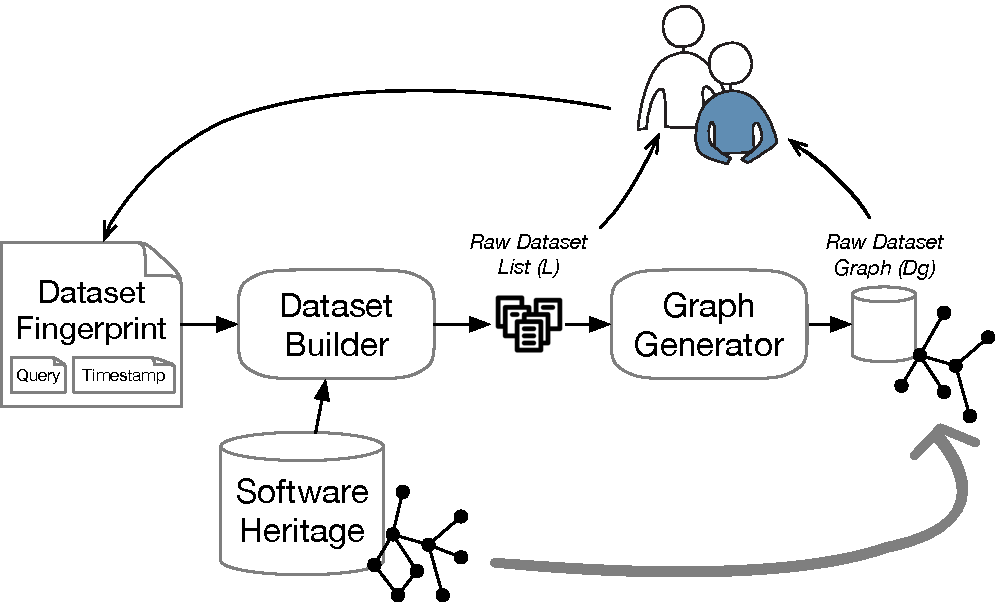
\includegraphics[width=0.4\textwidth]{images/appraoch.pdf}
    \vspace{-5 pt}

    \caption{Approach Overview}
    \label{fig:appraoch} 
    \vspace{-1.5 em}

\end{figure}

The \textbf{query specification} acts as a filter by defining constraints a repository must verify to be included in the output dataset.
These constraints are expressed over the repositories' metadata as defined in the unifying domain model of the SWH Graph Dataset (presented in the form of a class diagram in Figure~\ref{fig:swhModel}, which will be detailed later).
The expressivity of possible queries is thus bounded to that model. 
For instance, it is not possible to specify a query according to the content of the artifacts, because this metadata is not included in the domain model. 
Note that the SWH model provides the commonalities among the various original forges, but misses the specificities of each one (e.g., stars in GitHub and GitLab). 
While this information is included in the related SWH archive, filtering repositories based on such specificities thus requires a post-processing operation on the extracted dataset.

The \textbf{timestamp} is a unique identifier referring to a specific version of the SWH Graph Dataset. This timestamp ensures reproducibility since each version of the SWH Graph Dataset is immutable, and the versions are append-only over the time. Hence, it is possible, at any point in time, to retrieve the dataset from the version of the SWH Graph Dataset corresponding to the timestamp, or any subsequent versions. This ensures reproducibility of the dataset even if there is further changes in the code base (e.g. Git history rewriting, branch deletion, etc.). 

The result of this process is a list of SWHIDs referring to repositories matching the query and the timestamp (cf. \emph{Raw Dataset List} in Fig. \ref{fig:appraoch}).
This list of SWHIDs can be fed to a \emph{Graph Generator} which extracts the subset of the SWH Graph Dataset corresponding to these identifiers (cf. \emph{Raw Dataset Graph} in Fig. \ref{fig:appraoch}).
Consequently, the obtained dataset of repositories can be further manipulated with the same SWH infrastructure and programming interface.
For instance, it can be used later on as input of our approach to filter out elements according to a more restrictive fingerprint. 
It can also enable to filter and download specific files, instead of cloning all the repositories to extract only a few files from them during the data extraction phase, which follows the repository selection phase~\cite{vidoni2022systematic}.

To sum up, our approach can be defined as the following function:
\[ SWHg \times FP \rightarrow L \rightarrow Dg \]
where $SWHg$ is the SWH Graph Dataset, $FP$ a dataset fingerprint, $L$ the list of origin ID's matching $FP$, and  $Dg$ the resulting dataset in the form of a subset of the SWH Graph Dataset.

Although our approach rely on SWH, we propose a generic approach that can be applied to any forges that provide an immutability property and a way to query the metadata of its repositories.
